\documentclass{ximera}
\title{What is Ximera?}
\outcome{Understand what Ximera is and how it can be used}
\begin{document}
\begin{abstract}
An introduction to the Ximera system.
\end{abstract}
\maketitle

\href{http://ximera.osu.edu}{\sf Ximera}
is an open-source software project that
seeks to help course instructors create learning materials
for their students in the form of interactive
web pages and high quality PDF documents.
Our strategy to achieve this goal is to separate
content from deployment.

An author writes content as a \LaTeX\ document.
This produces a PDF handout that can be distributed to students.
Next the author uploads the same \LaTeX\ file to
\href{http://github.com}{\tt github.com},
a free web-based service providing a number of features
to developers and authors.
In turn \href{http://github.com}{\tt github.com} delivers
the file to the \href{http://ximera.osu.edu}{\sf Ximera}
interpreter, which posts the file on the web.
The web page has essentially the same content as the handout.
However, the web page typically has interactive features
not possible in the handout due to the physical limitations of paper.
For example, the web page might pose a question
that if answered incorrectly, would offer hints or further questions
to the student.
This process is illustrated in the figure below.

\begin{image}
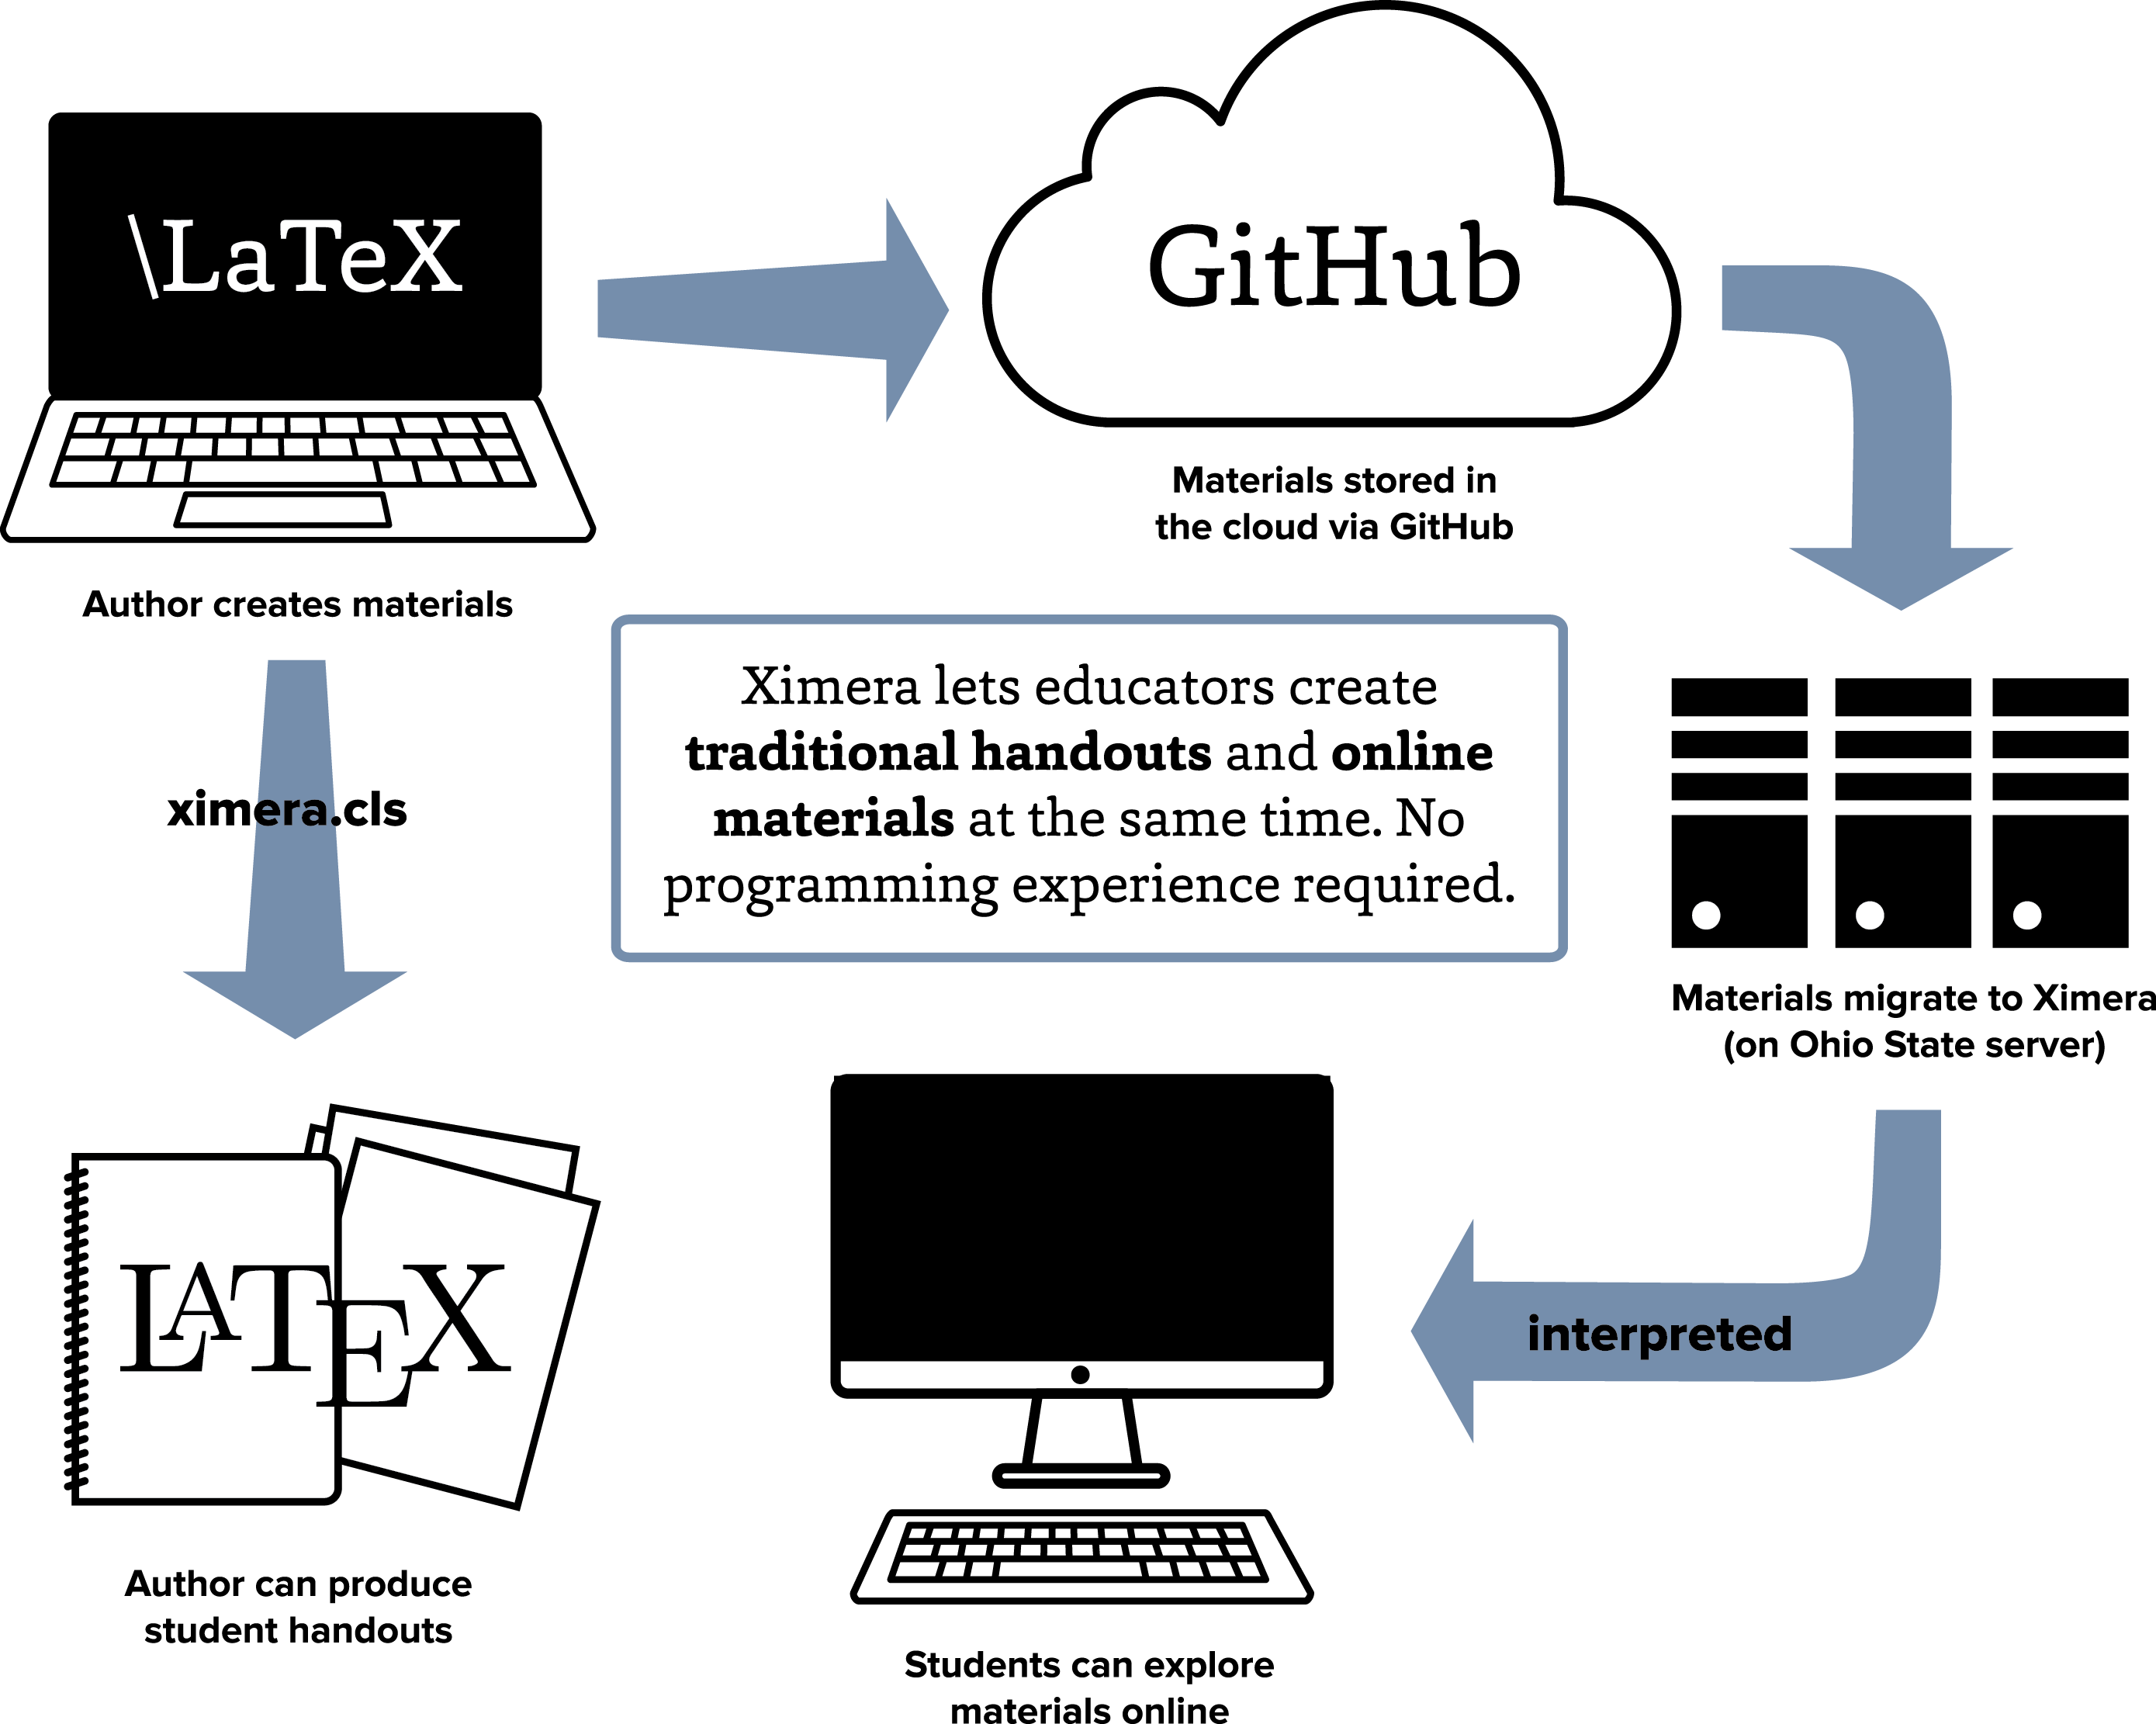
\includegraphics[scale=.25]{XimeraGraphic.png}
\end{image}

\subsection{Benefits of Ximera}
One benefit of \link[\sf Ximera]{http://ximera.osu.edu}
is that it provides an easy way to produce interactive online materials.
Another benefit is that many educators, particularly mathematicians,
are already quite familiar with \LaTeX\ and
even find it easy to use.
And because the \TeX\ language is extremely static in comparison with
other programming and markup languages, authors can expect
the \href{http://ximera.osu.edu}{\sf Ximera}
materials they create to be usable in some
form for the foreseeable future.

\subsection{Differences between Ximera and Learning Management Systems}
A Learning Management System
(LMS) such as Blackboard or Moodle
provides students with a central webpage from
which they can navigate to the webpage of
each of their courses, these course web pages
all formatted and laid out in exactly the same way.
Because of the possibility of conveying grades
to students, an LMS requires students
and instructors to have accounts,
which are typically set up by
the college or University, as are the course
web pages themselves.

By far, the most common way to use an LMS in our
experience is to make announcements or to distribute
files to students.  While this could be accomplished through email
or simple web pages, the LMS, being
largely set up by the college or University, provides
an even easier way to distribute files and communicate with students.
It also organizes students' course materials in a single location.

The function of an LMS most relevant to our discussion
of \href{http://ximera.osu.edu}{\sf Ximera} is assessment.
Instructors compose quizzes or homework assignments,
which consist of sequences of questions of various types.
Typically each question has a unique answer, allowing
the LMS to score the assignment and record grades in a
gradebook, another function of an LMS.
It should be born in mind that composing questions for
an LMS, particularly multiple-choice questions, creates a lot of work
for instructors. For this reason textbook publishers
are increasingly bundling their books with accounts
on proprietary LMS's, from which an
instructor can select precomposed exercises for students
to complete.

In contrast \href{http://ximera.osu.edu}{\sf Ximera}
provides a more flexible environment for creating course materials.
While an activity on an LSM consists solely of a sequence
of problems, a \href{http://ximera.osu.edu}{\sf Ximera}
activity can contain whatever content a \LaTeX\ document
can contain, and in addition, can include interactive questions
of various types.

\subsection{Ways Ximera can be used}
Whereas an LMS typically only supplements a traditional course,
an entire course can be delivered through
\href{http://ximera.osu.edu}{\sf Ximera}.
For example, a course could consist of a sequence
of \href{http://ximera.osu.edu}{\sf Ximera}
activities, each of which primarily composed of text
for students to read, with an occasional 
question sprinkled in to confirm and deepen students'
understanding of the material presented just before the question.
More substantial questions could appear at the end of the activity.

Another possibility is to use \href{http://ximera.osu.edu}{\sf Ximera}
in conjunction with a traditional lecture-based course,
using \href{http://ximera.osu.edu}{\sf Ximera}
to deliver pre-lecture reading materials and exercises
to be completed by students before arriving to their lecture.
These could serve as a prelude to the lecture,
perhaps presenting background topics or materials
to review before the lecture.

The emphasis of \href{http://ximera.osu.edu}{\sf Ximera}
is more on content delivery than on assessment.
We understand however that many students function
better knowing that their actions will be acknowledged by
their instructors. We therefore envisage providing ways
for instructors to access student scores on 
\href{http://ximera.osu.edu}{\sf Ximera} activities
in the near future. In the meantime it might
be better to use a traditional LMS to deliver exercises
if keeping track of student participation is important.

\end{document}
